\expandafter\newcommand\csname dataKNeighborsClassifiermetrictab\endcsname{
\begin{table}[H]
\begin{tabular}
{| 
 p{\dimexpr0.2\textwidth-2\tabcolsep-\arrayrulewidth\relax}| 
 p{\dimexpr0.2\textwidth-2\tabcolsep-\arrayrulewidth\relax}| 
 p{\dimexpr0.2\textwidth-2\tabcolsep-\arrayrulewidth\relax}| 
 p{\dimexpr0.2\textwidth-2\tabcolsep-\arrayrulewidth\relax}| 
 p{\dimexpr0.2\textwidth-2\tabcolsep-\arrayrulewidth\relax}| 
}\hline 
\textbf{} &\textbf{f1-score} &\textbf{precision} &\textbf{recall} &\textbf{support} \\ \hline 
CANDIDATE &0.29 &0.435 &0.218 &170.0 \\ \hline 
CONFIRMED &0.43 &0.416 &0.444 &241.0 \\ \hline 
FALSE POSITIVE &0.646 &0.598 &0.703 &391.0 \\ \hline 
accuracy &0.522 &0.522 &0.522 &0.522 \\ \hline 
macro avg &0.455 &0.483 &0.455 &802.0 \\ \hline 
weighted avg &0.506 &0.509 &0.522 &802.0 \\ \hline 
\end{tabular} 
\end{table}
}
\begin{figure}[H]
                \centering
                \begin{subfigure}{.49\textwidth}
                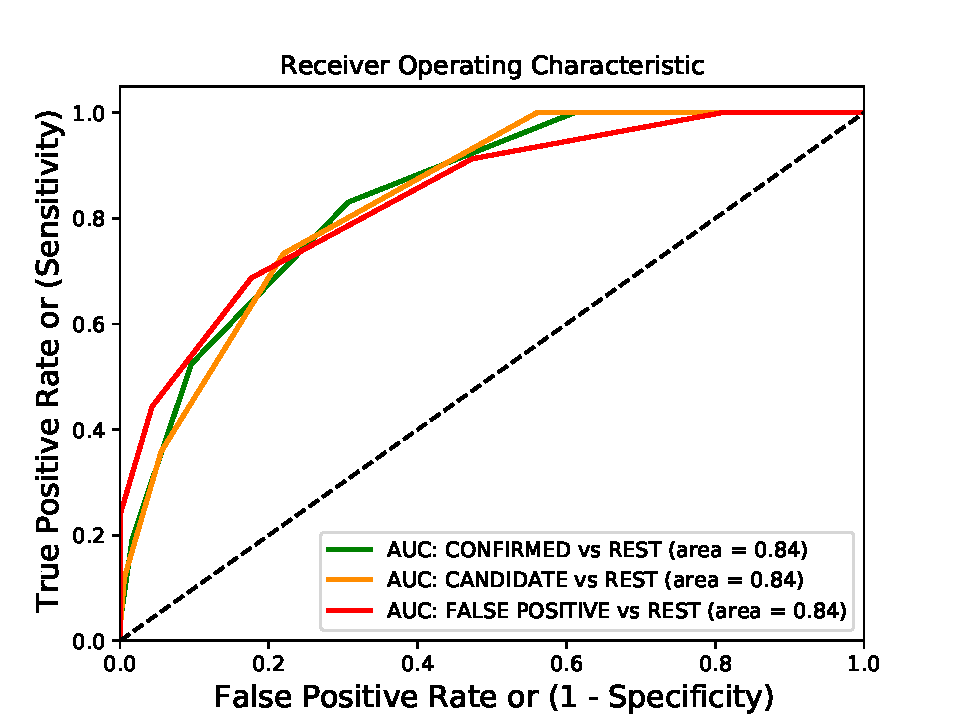
\includegraphics[width = 1\textwidth]{data/KNeighborsClassifier_overfit_roc.pdf}
                \end{subfigure}
                \begin{subfigure}{.49\textwidth}
                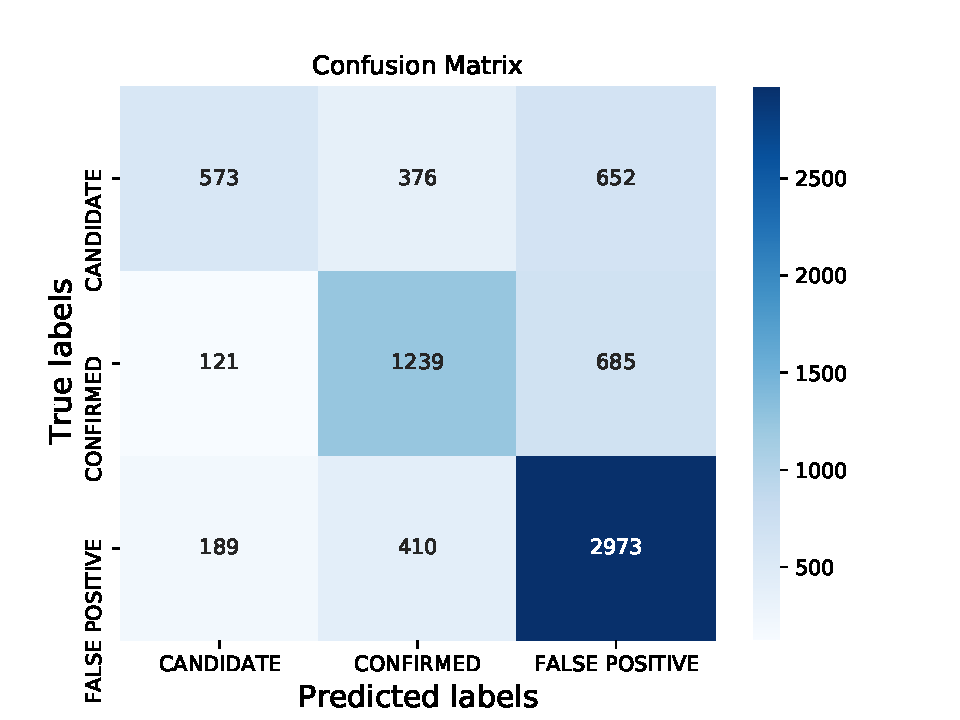
\includegraphics[width = 1\textwidth]{data/KNeighborsClassifier_overfit_cm.pdf}
                \end{subfigure}
                \begin{subfigure}{.49\textwidth}
                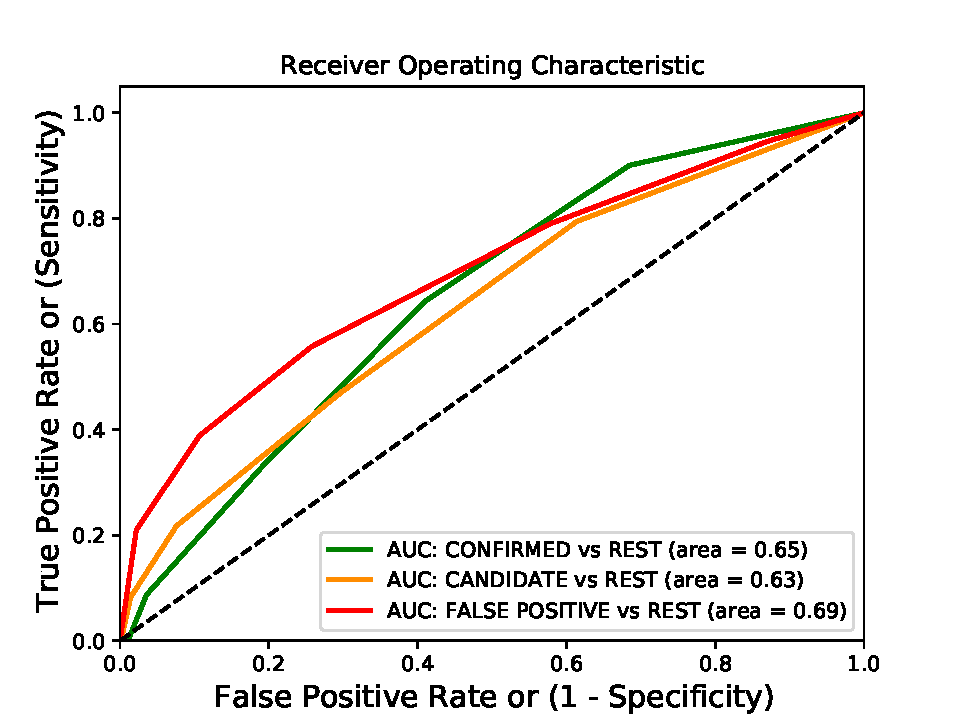
\includegraphics[width = 1\textwidth]{data/KNeighborsClassifier_roc.pdf}
                \end{subfigure}
                \begin{subfigure}{.49\textwidth}
                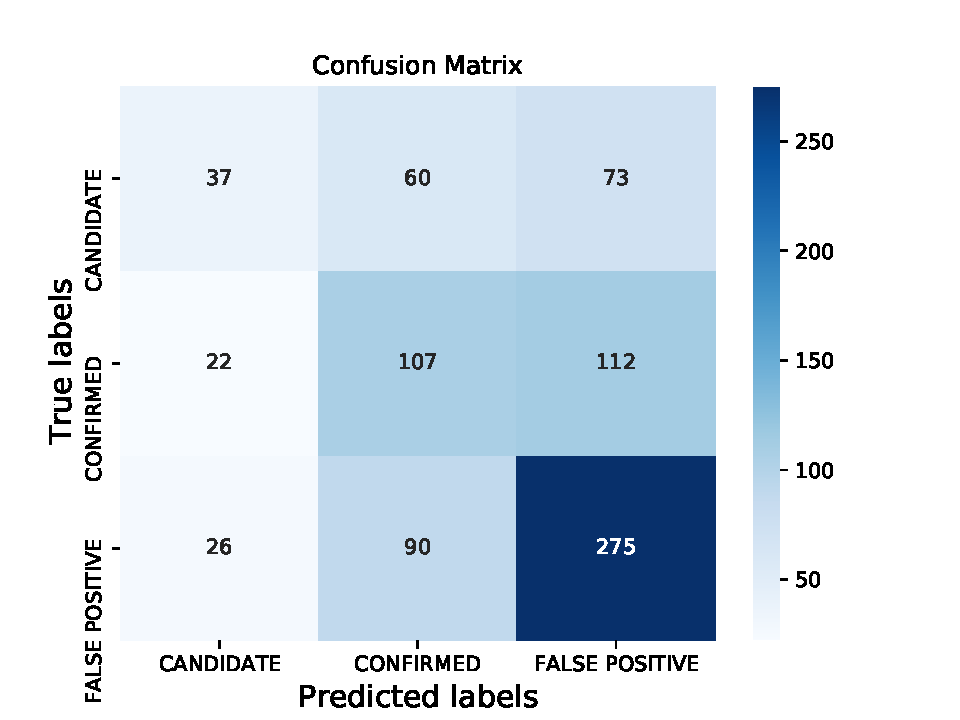
\includegraphics[width = 1\textwidth]{data/KNeighborsClassifier_cm.pdf}
                \end{subfigure}
                \begin{subfigure}{1\textwidth}
                \csname dataKNeighborsClassifiermetrictab\endcsname
                \end{subfigure}
                \caption{KNeighborsClassifier: Top Row: overfit test. Middle and bottom row test data}
                \label{fig:data/KNeighborsClassifier_roc}
                \end{figure}